\chapter{Deseño de software}
O longo deste capítulo detállase a arquitectura do sistema a desenvolver. Mostrase primeiro a arquitectura xeral e a súa interacción con sistemas externos e posteriormente detallase máis polo miúdo a estrutura dos distintos compoñentes do sistema.

\section{Arquitectura do sistema}
Xa na definición dos obxectivos do sistema se identifican dúas partes diferenciadas dentro do sistema. Por un lado a comunicación co servidor SOS, para a obtención dos datos de observacións, e por outro a visualización e explotación destes datos. Esta diferenciación trasládase directamente á arquitectura do sistema, que se divide en dous compoñentes. Na figura \ref{fig:diaComponentes} represéntanse estes dous subsistemas, acompañados polos demais sistemas externos dos que dependen.

\begin{figure}[hbtp]
 \centering
 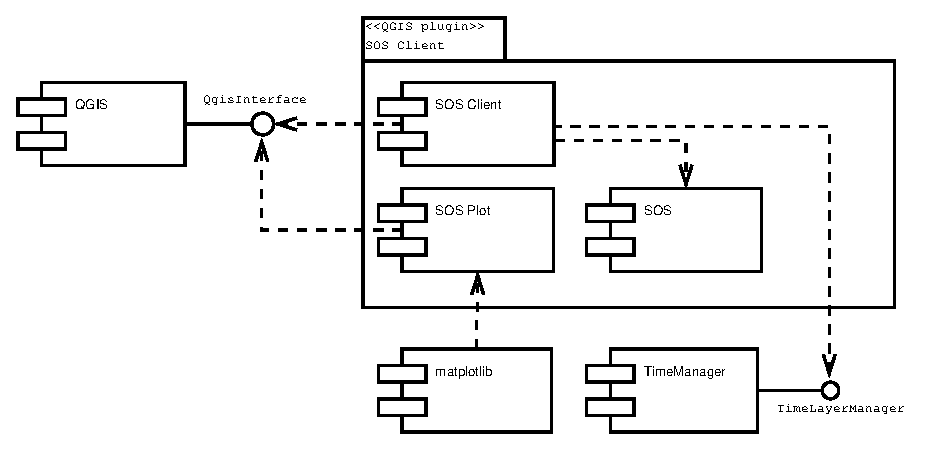
\includegraphics[width=\textwidth]{images/componentes.eps}
 \caption{Diagrama de compoñentes}
 \label{fig:diaComponentes}
\end{figure}

\begin{sidewaysfigure}
 \centering
 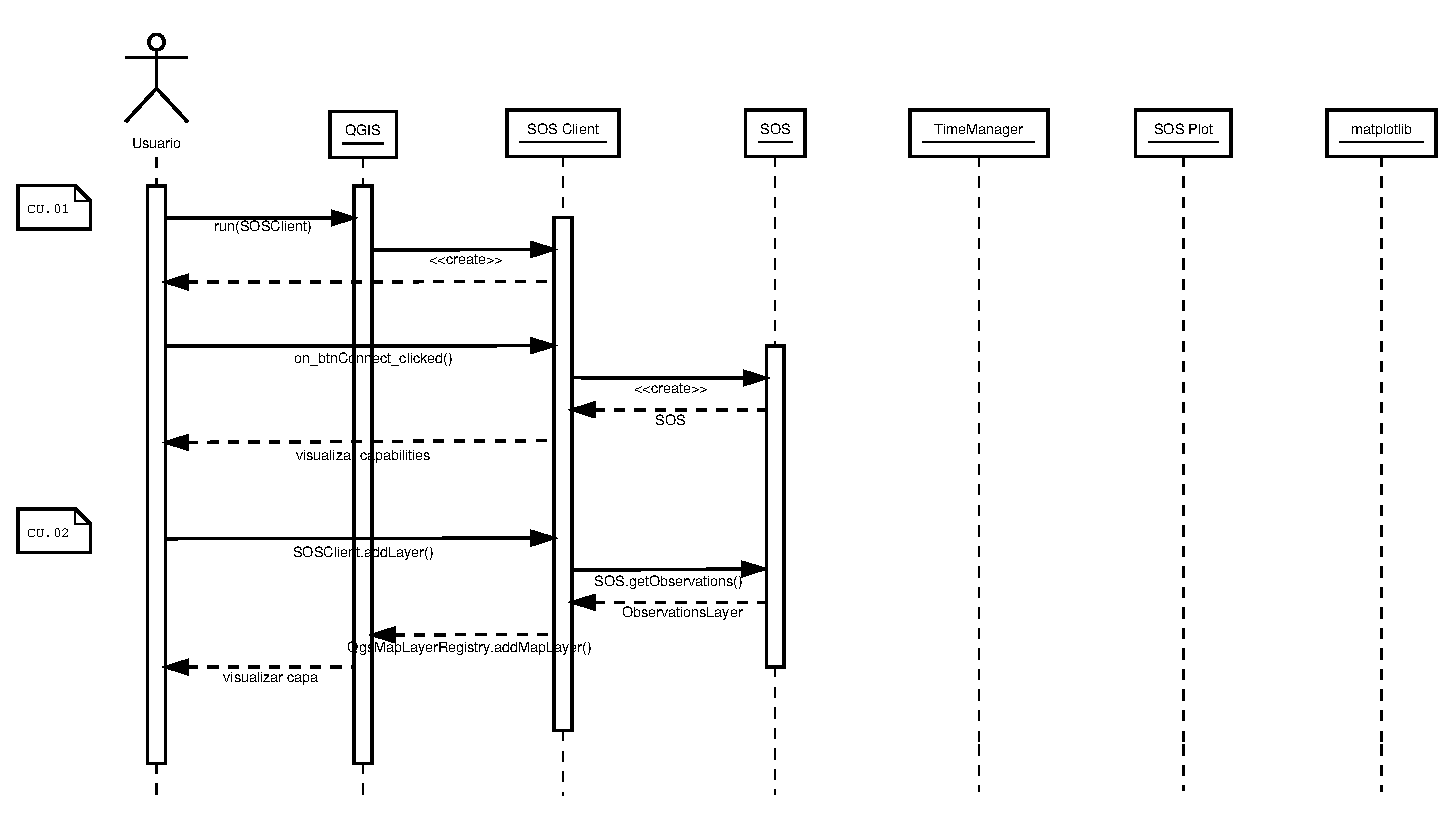
\includegraphics[width=\textwidth]{images/seq1.eps}
 \caption{Diagrama de secuencia para os casos de uso \ref{uc:CU.01} e \ref{uc:CU.02}}
 \label{fig:diaSeq1}
\end{sidewaysfigure}

\begin{sidewaysfigure}
 \centering
 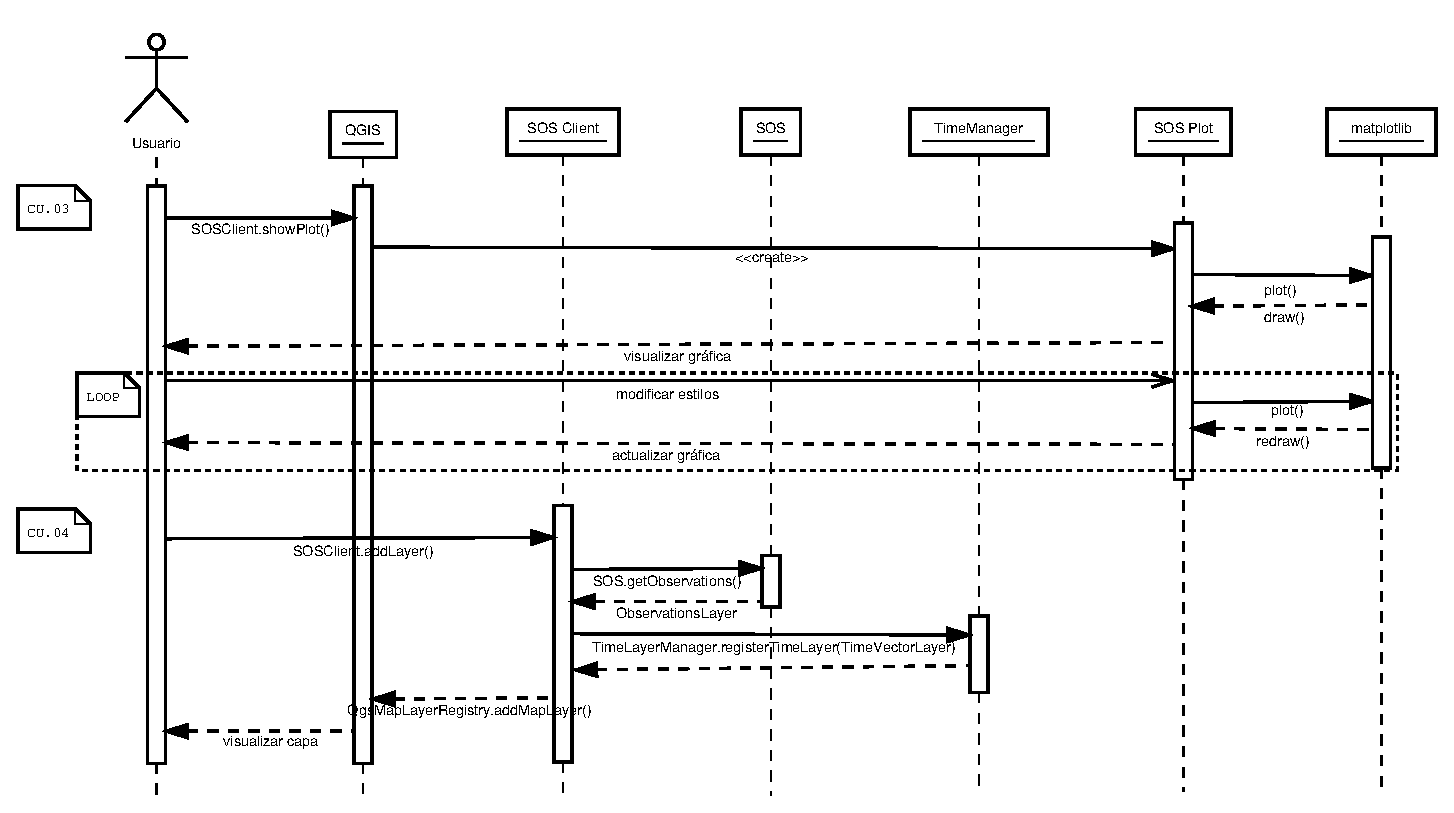
\includegraphics[width=\textwidth]{images/seq2.eps}
 \caption{Diagrama de secuencia para os casos de uso \ref{uc:CU.03} e \ref{uc:CU.04}}
 \label{fig:diaSeq2}
\end{sidewaysfigure}

\begin{sidewaysfigure}
 \centering
 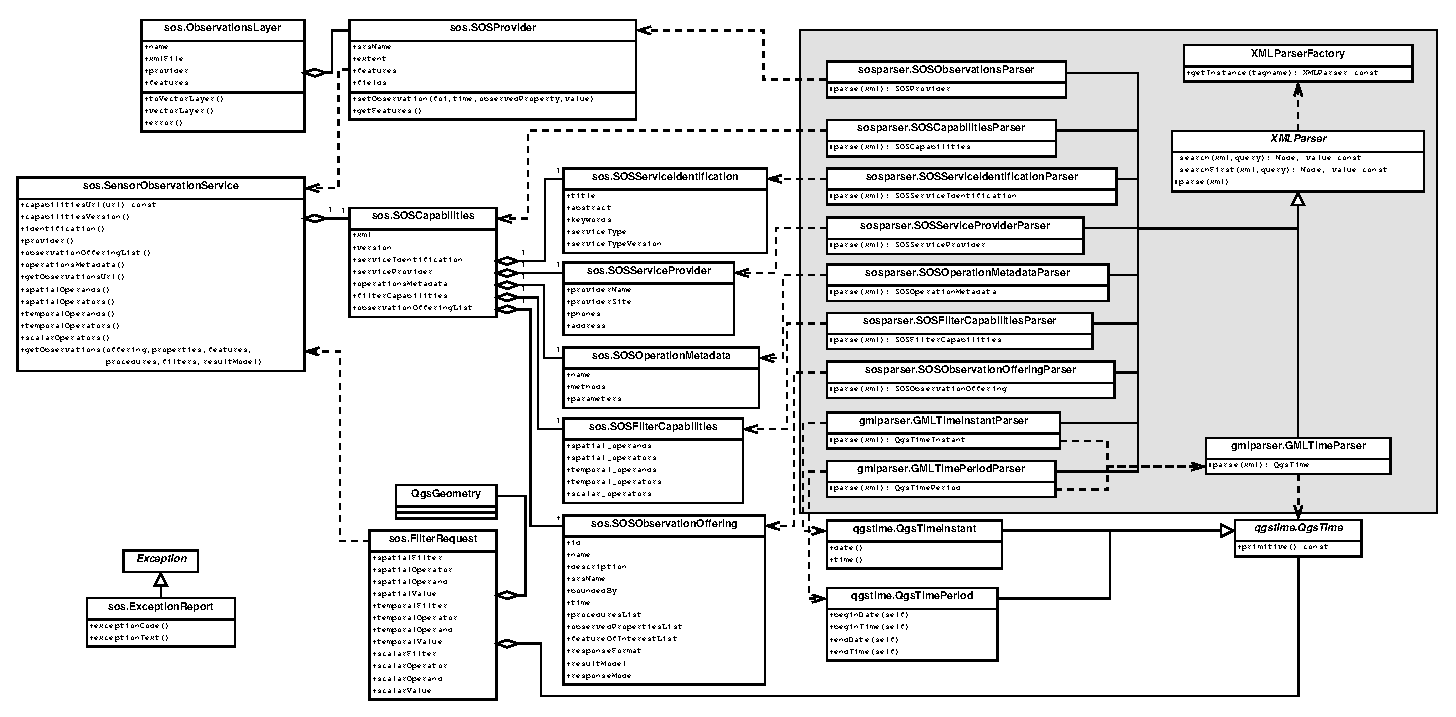
\includegraphics[width=\textwidth]{images/clases_sos.eps}
 \caption{Diagrama de clases}
 \label{fig:diaClassSOS}
\end{sidewaysfigure}


Deseño: cómo se realiza o Sistema, a división deste en diferentes compoñentes e a comunicación entre eles. Así mesmo, determinarase o equipamento hardware e software necesario, xustificando a súa elección no caso de que non fora un requisito previo. Debe achegarse a un nivel suficiente de detalle que permita comprender a totalidade da estrutura do produto desenvolvido, utilizando no  posible representacións gráficas.

WIP